\documentclass{article}
\RequirePackage[a4paper,top=.5cm,left=.5cm,right=.5cm,bottom=.5cm]{geometry}

\usepackage{pdfpages}
\usepackage{fp}% http://ctan.org/pkg/calc
\usepackage{tikz}
\begin{document}

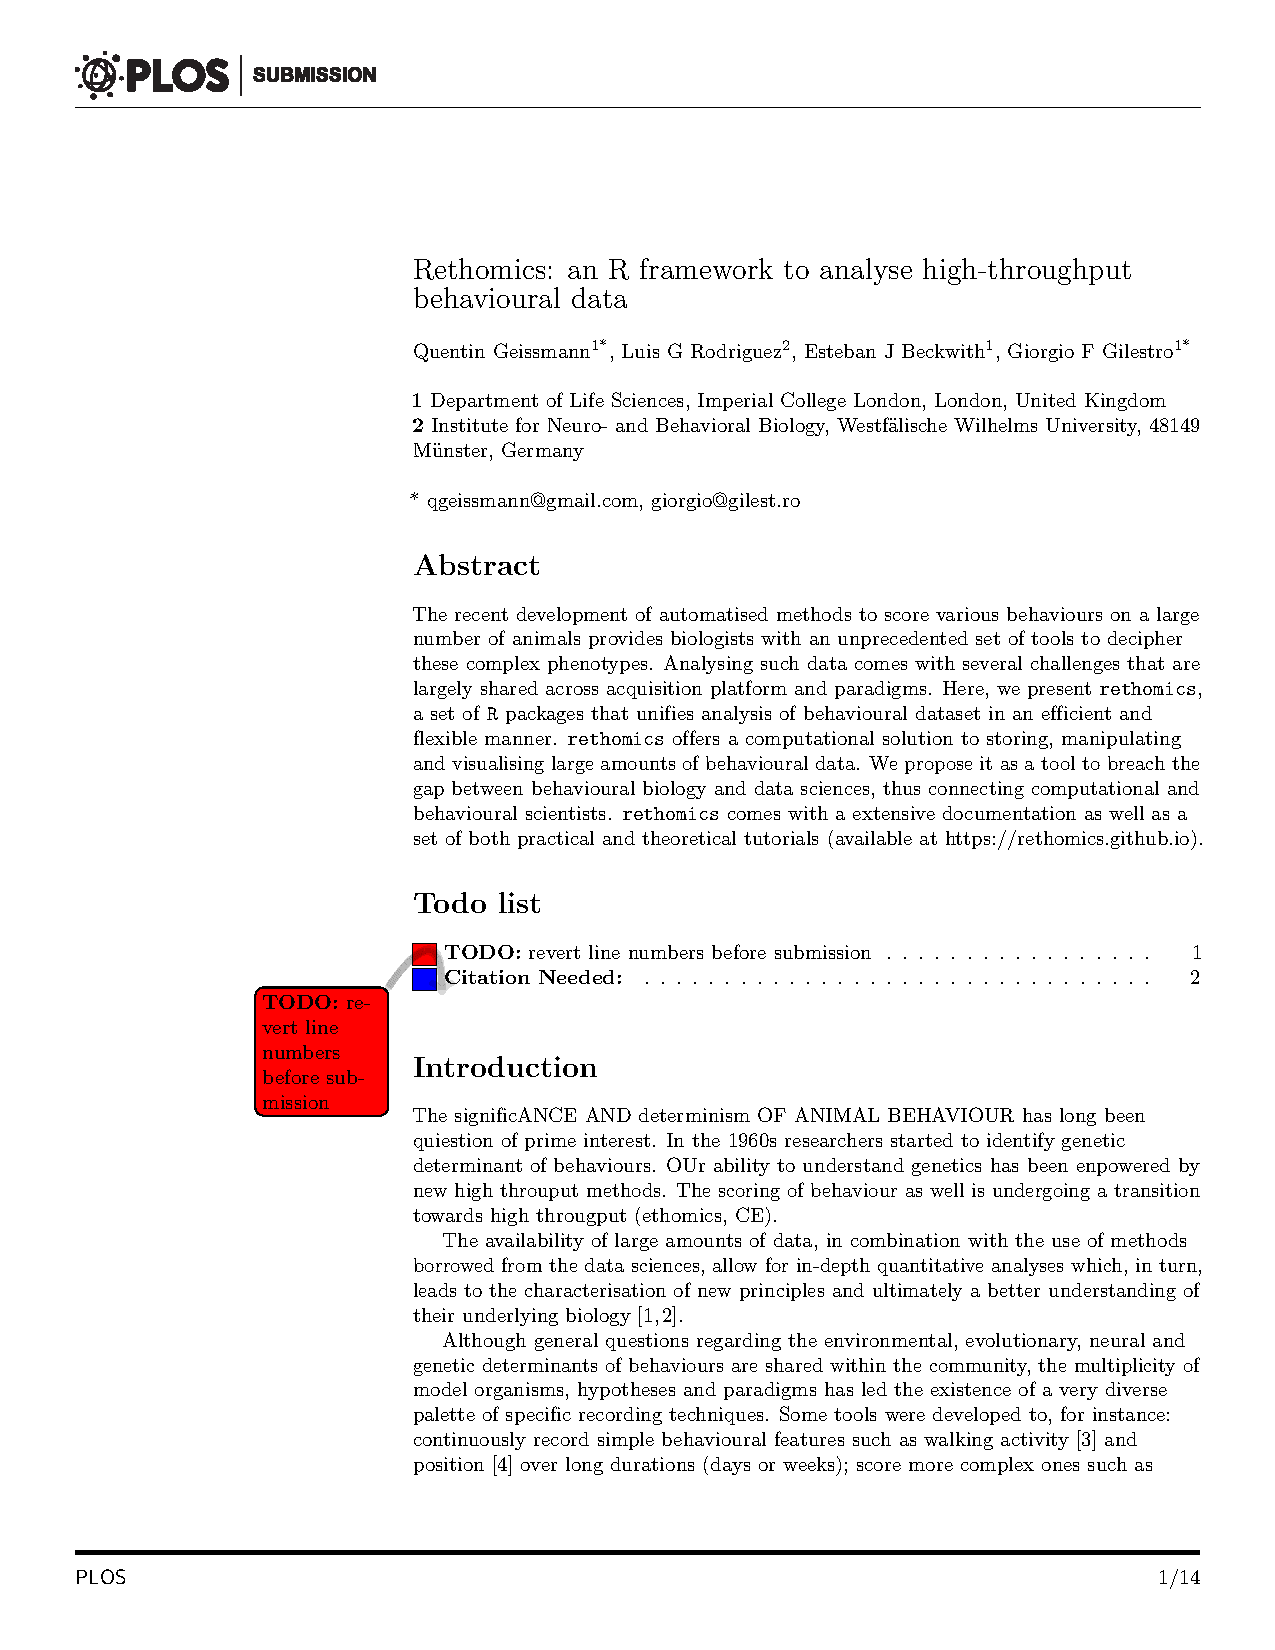
\includepdf[pages=1-]{manuscript.pdf}

\foreach \x in {1,2,3,4,5}
{ 	\begin{figure}[h!]
		\centering   
		\includegraphics[width=.90\textwidth, page=\x]{all-figures.pdf}
	\end{figure}
	\vspace*{\fill}
	\textbf{\LARGE{Geissmann et al. 2018, Fig \x}}
	\clearpage
}	

\foreach \x in {6}
{ 	\begin{figure}[h!]
		\centering   
		\includegraphics[width=.90\textwidth, page=\x]{all-figures.pdf}
	\end{figure}
	\vspace*{\fill}
	\FPeval{\result}{clip(\x-5)}
	\textbf{\LARGE{Geissmann et al. 2018, Fig S\result}}
	\clearpage
}		

\end{document}